\chapter{予備実験と考察}

本章では，第 4 章で述べた評価基盤を用いて実施した予備実験について述べる．5.1 節で目的と設定を示し，5.2 節で結果を報告する．5.3 節で差の統計的な検証を行い，5.4 節で結果を考察し，5.5 節で本研究の限界を整理する．

本章に示す数値は，4.4 節で述べた採点処理の修正を反映したものである．

\section{実験の目的と設定}

予備実験の目的は 2 つである．第一に，構築した評価基盤が意図通りに動作することを確認すること，第二に，3 つの引き出し方式の間に較正の差が現れるかを把握することである．差の大きさが分かれば，本実験で必要な問題数の検討に使える．ただし1 モデル・1 領域での単一試行であり，結果から一般的な結論を導くことは意図していない．設定は表 3.2 に示した通りで，3 方式それぞれについて 250 問を実行し，合計 750 問分の応答を得た．

\section{結果}

3 方式の結果を表 5.1 に示す．

\begin{table}[htbp]
\centering
\small
\caption{3 方式の比較（日本語版 MGSM，250 問）}
\label{tab:5.1}
\scalebox{0.86}{
\begin{tabular}{|l|l|l|l|l|l|l|l|l|}
\hline
方式 & 採点対象 & 正答率 & ECE & Brier & AUROC & REL & RES & UNC \\
\hline
Verb.1S & 248 & 215/250 = 86.0\% & 0.0712 & 0.0978 & 0.738 & 0.0115 & 0.0287 & 0.1154 \\
Verb.2S & 250 & 221/250 = 88.4\% & 0.0438 & 0.0785 & 0.797 & 0.0070 & 0.0284 & 0.1025 \\
Ling.1S & 250 & 195/250 = 78.0\% & 0.1266 & 0.1733 & 0.629 & 0.0170 & 0.0153 & 0.1716 \\
\hline
\end{tabular}
}
\end{table}

正答率の分母は全 250 問である．一方 ECE，Brier Score，AUROC，Murphy 分解は確信度が取得できた問題のみで計算しており，その件数を「採点対象」列に示した．確信度の取得に失敗したのは Verb.1S の 2 問のみである．なお 3.4 節で述べたとおり，REL − RES + UNC は区間に集約した予測に対する Brier Score に対応し，表中の Brier Score とは一般に一致しない．実際の差は Verb.1S で −0.0003，Verb.2S で −0.0026 であり，Ling.1S では 0 である．

正答率，ECE，Brier Score，AUROC，REL の点推定では Verb.2S が最良で，RES の点推定は Verb.1S が最も高い．統計的な検証は 5.3 節で行う．

確信度の分布を図 5.1 に示す．分母はいずれも各方式の採点対象の件数である．3 方式のいずれにおいても，確信度が 0.9 以上の区間に偏っている．該当する件数はVerb.1S が 248 件中 225 件，Verb.2S が 250 件中 217 件，Ling.1S が 250 件中203 件である．Ling.1S では 5 段階のうち 4 段階が使われ，最上位の「ほぼ確実」が203 件と全体の 81.2\% を占めた．最下位の「ほとんどわからない」は 1 件も選ばれていない．

\begin{figure}[htbp]
\begin{center}
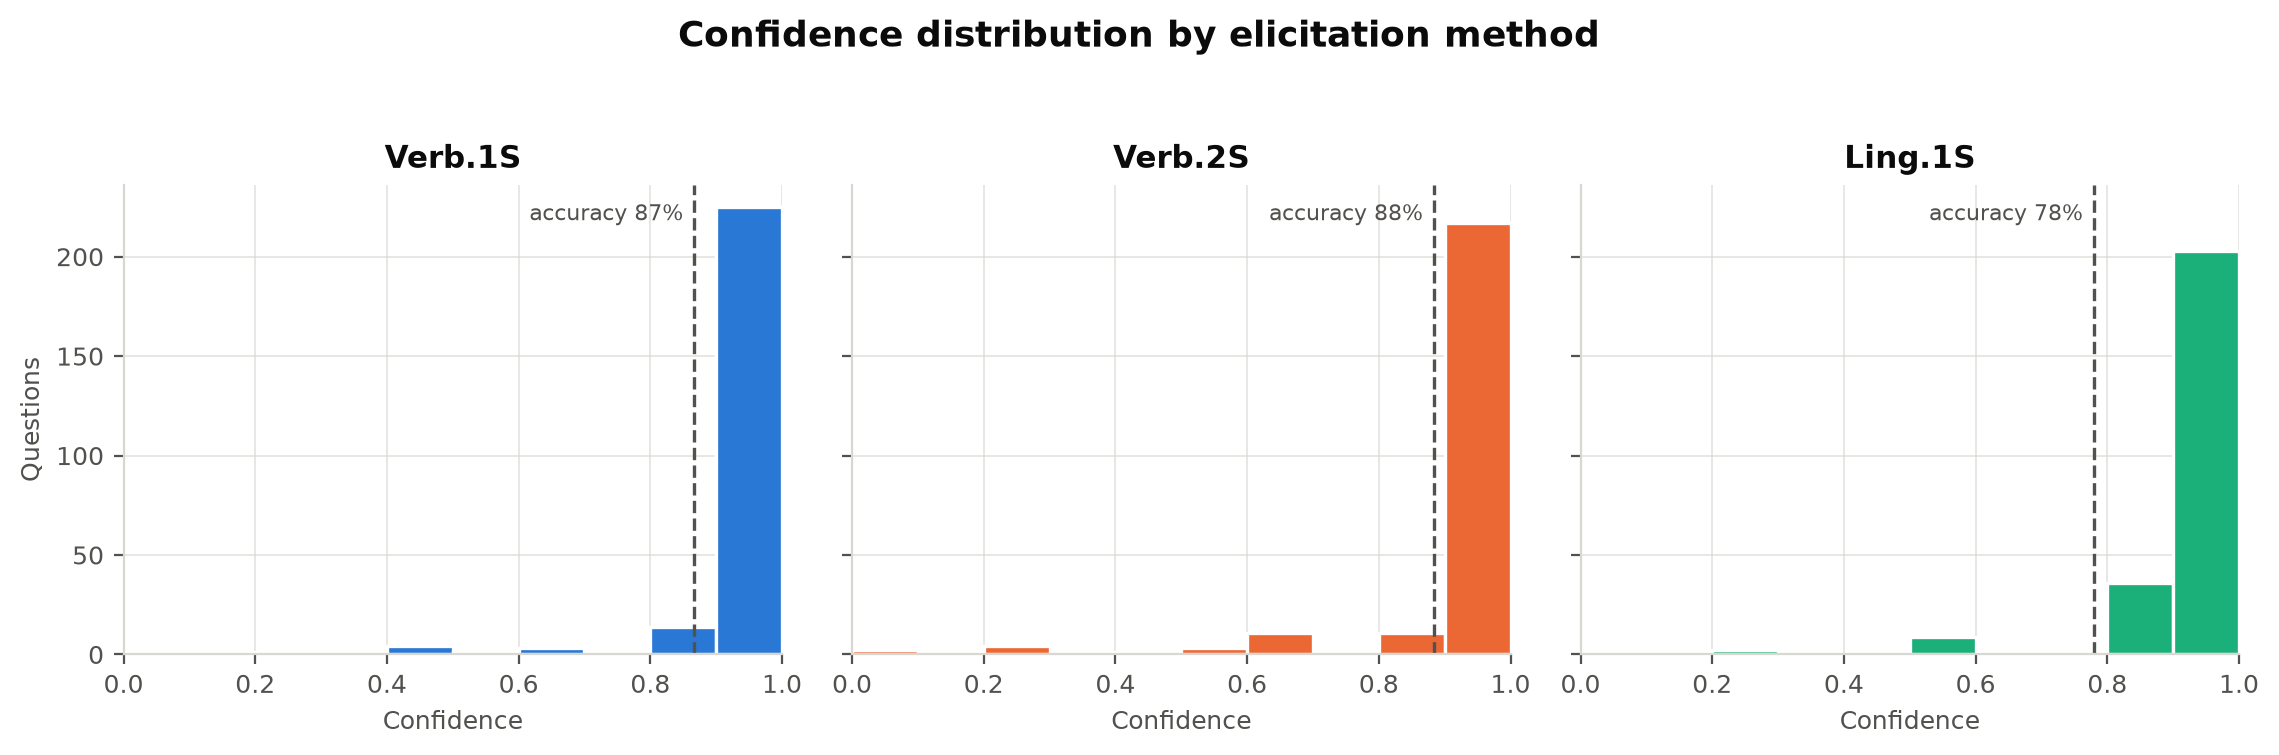
\includegraphics[width=12cm]{./figure/confidence-distribution.png}
\caption{確信度の分布（方式別）}
\label{fig:5.1}
\end{center}
\end{figure}

平均確信度と平均正答率を表 5.2 に示す．いずれも採点対象の件数を分母とする．

\begin{table}[htbp]
\centering
\small
\caption{平均確信度と平均正答率（採点対象のみ）}
\label{tab:5.2}
\begin{tabular}{|l|l|l|l|l|}
\hline
方式 & 採点対象 & 平均確信度 & 平均正答率 & 差 \\
\hline
Verb.1S & 248 & 0.938 & 0.867 & +0.071 \\
Verb.2S & 250 & 0.921 & 0.884 & +0.037 \\
Ling.1S & 250 & 0.907 & 0.780 & +0.127 \\
\hline
\end{tabular}
\end{table}

3 方式とも平均確信度は 0.91 から 0.94 の範囲にあり，差はいずれも正である．すなわちモデルは実際の正答率より高い確信度を表明しており，方式によって大きく変化したのは確信度ではなく正答率の側である．

確信度と正答率の対応を図 5.2 に示す．対角線は完全な較正に相当し，これより下側にある点は，その確信度帯において確信度が正答率を上回っていることを示す．

\begin{figure}[htbp]
\begin{center}
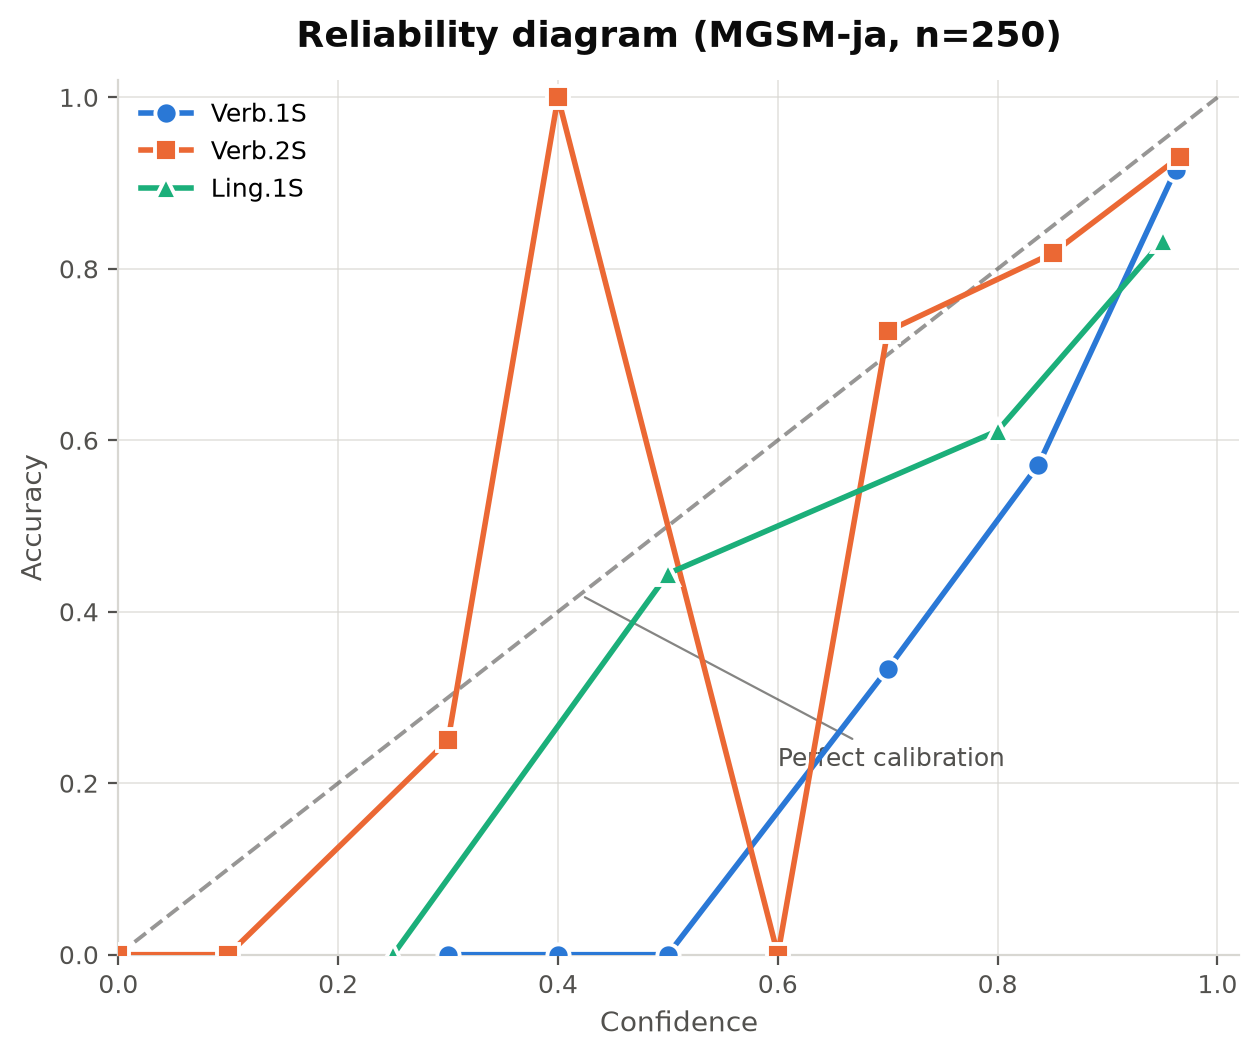
\includegraphics[width=9.5cm]{./figure/reliability-diagram.png}
\caption{信頼度ダイアグラム}
\label{fig:5.2}
\end{center}
\end{figure}

10 区間のうち標本が存在する区間は，Verb.1S で 6 個，Verb.2S で 8 個，Ling.1S で4 個である．低確信度側には 1 件ないし数件しか含まれない区間があり，そこでの区間正答率は少数の問題に左右される．折れ線はこの違いを表現しないため，低確信度帯の点は高確信度帯の点と同じ重みでは読めない．

\section{差の統計的検証}

表 5.1 の差が標本の揺らぎで説明できるかを確かめるため，問題の復元抽出による信頼区間を求めた．3 方式すべてで確信度が取得できた 248 問を対象とし，5000 回の再抽出を行った．4.3 節で述べたとおり，3 方式には同じ添字を適用する対応のある設計とした．対象が 248 問に揃うため，本節の点推定は表 5.1 の値とわずかに異なる．なお，以下は 18 通りの比較それぞれに対する個別の 95\% 信頼区間であり，多重比較の調整は行っていない．探索的な分析として扱う．

方式間の差の信頼区間を表 5.3 に示す．区間が 0 を含まない場合，その差は標本の揺らぎでは説明しにくい．該当する組み合わせには印を付けた．

\begin{table}[htbp]
\centering
\small
\caption{方式間の差の 95\% 信頼区間（共通 248 問，† は区間が 0 を含まない）}
\label{tab:5.3}
\scalebox{0.74}{
\begin{tabular}{|l|l|l|l|}
\hline
指標 & Verb.1S − Verb.2S & Verb.1S − Ling.1S & Verb.2S − Ling.1S \\
\hline
ECE & +0.029 [−0.014, +0.054] & −0.052 [−0.097, −0.012] † & −0.080 [−0.120, −0.031] † \\
Brier & +0.019 [−0.007, +0.047] & −0.073 [−0.109, −0.038] † & −0.092 [−0.129, −0.058] † \\
AUROC & −0.054 [−0.145, +0.030] & +0.112 [+0.012, +0.211] † & +0.166 [+0.048, +0.274] † \\
REL & +0.005 [−0.007, +0.017] & −0.004 [−0.019, +0.009] & −0.009 [−0.024, +0.003] \\
RES & +0.003 [−0.014, +0.019] & +0.015 [−0.001, +0.034] & +0.013 [−0.006, +0.033] \\
正答率 & −0.020 [−0.052, +0.012] & +0.081 [+0.036, +0.125] † & +0.101 [+0.056, +0.145] † \\
\hline
\end{tabular}
}
\end{table}

全 18 通りの比較のうち，8 通りで区間が 0 を含まなかった．主張できることは3 点に限られる．第一に，Ling.1S は他の 2 方式より ECE，Brier Score，AUROC，正答率で劣る．この 4 指標において，Ling.1S と他の 2 方式との差はいずれも区間が0 を含まなかった．第二に，REL と RES では差を検出できなかった．したがって，Ling.1S の較正が他の 2 方式より劣ることを REL の水準で示すことはできていない．ただし AUROC では差が検出されているため，識別に関わる性質全般について差がないとは言えない．第三に，Verb.1S と Verb.2S の差は 6 指標すべてで区間が 0 を含んだ．2 段階方式が 1 段階方式より優れているとは言えないが，これは差が存在しないことを示すものでもなく，今回の標本では検出できなかった，というのが正確な表現である．必要な標本数を見積もるには，実用上意味のある差の大きさを先に定める必要がある．

\section{考察}

予備実験で最も顕著だったのは，3 方式のいずれにおいても確信度が 0.9 以上に偏り，引き出し方を変えても分布がほとんど動かなかったことである．表 5.2 のとおり平均確信度は平均正答率を 0.037 から 0.127 上回っており，モデルが自信過剰であるという Xiong ら \cite{xiong2024llmuncertainty} の報告と整合する．3 方式とも AUROC の信頼区間は0.5 を上回っており，順序の情報が完全に失われているわけではない．しかし分布が偏っているため，確信度の値を手がかりに検証対象を絞り込む用途では，使える段階が実質的に限られる．

ただし，分布の偏りと較正の良否は別の事柄である．本実験の対象は算数の文章題であり，正答率は 78\% から 88\% と高い．正答率が高ければ高い確信度が多くなること自体は妥当であり，偏りが直ちに問題を意味するわけではない．問題は，偏りの程度が正答率の水準より強く，かつ方式を変えても分布がほとんど動かないことである．

この分布は指標の解釈にも影響する．表 5.1 の ECE と，表 5.2 の「平均確信度と平均正答率の差」はほぼ一致している（Verb.1S で 0.0712 と 0.071，Verb.2S で0.0438 と 0.037，Ling.1S で 0.1266 と 0.127）．これは，標本の大半が高確信度側の少数の区間に入っており，かつ多くの区間で確信度が正答率を上回っているために生じる．ECE は区間ごとの差の絶対値を重みづけて平均するため，差の符号が区間をまたいで揃っていれば，その値は全体の平均どうしの差に近づく．

このことは ECE が較正を測っていないことを意味しない．言えるのは，この分布のもとでは ECE の値だけを見て較正の良否と正答率の高低を読み分けることが難しい，ということである．たとえば Ling.1S の ECE が他より大きいことは，較正が劣るためとも，正答率が低いためとも読める．当初の研究計画では Murphy 分解の REL を用いればこの読み分けができると考えていたが，これは誤りであった．3.4 節で述べたとおり REL は各区間の正答率を含み，実測でも 3 通りの比較すべてで信頼区間が0 を含んでいる．したがって本研究は現時点で，第 1 章に挙げた第 2 の問いに答えられていない．答えるには指標の選択ではなく実験の設計を変える必要がある．具体的には，ある方式で得られた回答を全方式に共通の回答として与え，それに対する確信度のみを尋ねれば，正誤ラベルが共通になるため較正の違いだけを取り出せる．この経緯から得られる方法論上の知見として，較正を報告する際には確信度の分布を併記すべきである．分布が偏っている場合，ECE の値は平均どうしの差に近づくため，値だけを他の研究と比較しても意味を読み違えうる．

もう 1 つ注目すべきは，Ling.1S の正答率が 78.0\% であり，他の 2 方式を 8 ポイントから 10 ポイント下回った点である．3 方式が解く問題も対象モデルも同一であり，違いは確信度の尋ね方だけである．確信度の引き出しは回答に対して中立な操作であると暗黙に仮定されがちだが，この結果はその仮定が成り立たない場合があることを示している．原因は特定できていないが，言語表現の提示によってプロンプトが長くなり問題への注意が薄れた可能性などが考えられる．なお，この差の大きさは採点処理の修正によって 12〜15 ポイントから 8〜10 ポイントへ縮小した．回答の抽出に関わる不具合が Ling.1S に偏って発生していたためであり，採点処理の詳細が方式間の比較に影響しうることは記録しておく必要がある．

\section{本研究の限界}

現時点での限界を 4 点に整理する．

第一に，対象が 1 モデル・1 領域での単一試行に限られる．他のモデルや他の領域で同じ傾向が得られるかは確認できていない．また MGSM は英語で作成された問題を翻訳したものであるため，日本固有の知識を含む課題への一般化も確認できていない．同一条件を複数回実行した場合の再現性も確認しておらず，問題の再抽出による信頼区間はモデル出力の揺らぎを評価するものではない．

第二に，3 方式は回答そのものが異なるため，較正の違いと正答率の違いを分離できていない．

第三に，言語表現と数値の対応づけが暫定的であり，表 3.1 の割り当てが変わればLing.1S の ECE，Brier Score，REL は変化する．

第四に，採点処理の検証が完全ではない．4.4 節の 2 件の不具合は，指摘された事例と同じ形式のものを探した範囲で修正したものである．また Verb.2S は第 1 ターンの応答を保存しておらず，回答の抽出に関わる検証が非対称である．
